\documentclass{standalone}
\usepackage{tikz}
\begin{document}
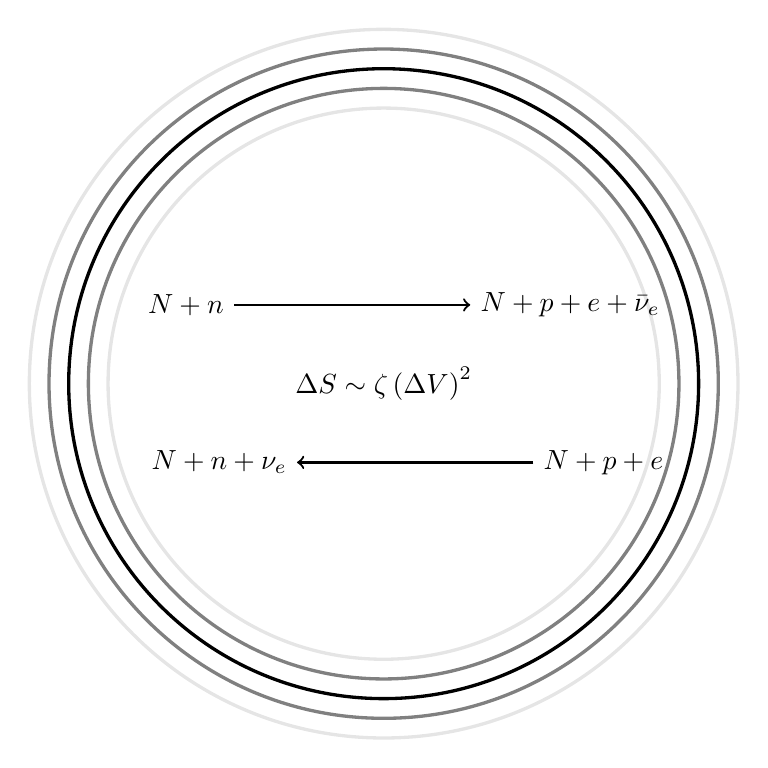
\begin{tikzpicture}
    \draw[very thick](0,0) circle (4);
    \draw[color=black!50, very thick](0,0) circle (3.75);
    \draw[color=black!10, very thick](0,0) circle (3.5);
    \draw[color=black!50, very thick](0,0) circle (4.25);
    \draw[color=black!10, very thick](0,0) circle (4.5);
    \draw[thick, ->] (-1.9, 1) node[left]{$N+n$}  -- ( 1.1, 1) node[right]{$N+p+e+\bar{\nu}_e$};
    \draw[thick, ->] ( 1.9,-1) node[right]{$N+p+e$} -- (-1.1,-1) node[left]{$N+n+\nu_e$};
    \node[] at (0,0) {$\Delta S \sim \zeta \left(\Delta V\right)^2$};
    \end{tikzpicture}
\end{document}

